\documentclass[12pt, a4paper]{book}

\usepackage[T1]{fontenc}
\usepackage[utf8]{inputenc}
\usepackage[charter, cal=cmcal]{mathdesign}
\usepackage[scaled=0.92]{helvet}
\usepackage{geometry}
\geometry{a4paper, top=30mm, bottom=30mm, inner=32mm, outer=25mm, marginparwidth=18mm}

\usepackage{amsmath, amsthm}
\usepackage[version=4]{mhchem}
\usepackage{graphicx}
\usepackage{xcolor}
\usepackage{tikz}
\usetikzlibrary{arrows.meta, shapes.geometric, positioning, calc, backgrounds}
\usepackage{pgfplots}
\pgfplotsset{compat=1.18}
\usepackage{tcolorbox}
\tcbuselibrary{skins, breakable, theorems}
\usepackage{titlesec}
\usepackage{fancyhdr}
\usepackage{enumitem}
\usepackage{booktabs}
\usepackage{array}
\usepackage{parskip}
\usepackage{siunitx}
\usepackage[colorlinks=true, linkcolor=BrickRed,
            urlcolor=NavyBlue, citecolor=ForestGreen]{hyperref}

% ── Colours (Journey 8 — forest green / amber) ────────────────────────────────
\definecolor{JourneyColor}{HTML}{065F46}
\definecolor{ModuleColor}{HTML}{059669}
\definecolor{PuzzleColor}{HTML}{B45309}
\definecolor{DiscoveryColor}{HTML}{D97706}
\definecolor{WarningColor}{HTML}{991B1B}
\definecolor{ProblemColor}{HTML}{6B21A8}
\definecolor{ReflectColor}{HTML}{0D9488}
\definecolor{HistoryColor}{HTML}{78350F}

% ── Boxes ─────────────────────────────────────────────────────────────────────
\newtcolorbox{puzzlebox}[1][]{enhanced,breakable,
  colback=PuzzleColor!6,colframe=PuzzleColor,fonttitle=\bfseries\sffamily,
  title={The Puzzle},attach boxed title to top left={yshift=-2mm,xshift=6mm},
  boxed title style={colback=PuzzleColor},borderline west={3pt}{0pt}{PuzzleColor},#1}

\newtcolorbox{discoverybox}[1][]{enhanced,breakable,
  colback=DiscoveryColor!8,colframe=DiscoveryColor,fonttitle=\bfseries\sffamily,
  title={Discovery},attach boxed title to top left={yshift=-2mm,xshift=6mm},
  boxed title style={colback=DiscoveryColor},borderline west={3pt}{0pt}{DiscoveryColor},#1}

\newtcolorbox{problembox}[1][]{enhanced,breakable,
  colback=ProblemColor!5,colframe=ProblemColor,fonttitle=\bfseries\sffamily,
  title={Problems},attach boxed title to top left={yshift=-2mm,xshift=6mm},
  boxed title style={colback=ProblemColor},borderline west={3pt}{0pt}{ProblemColor},#1}

\newtcolorbox{deepbox}[1][]{enhanced,breakable,
  colback=JourneyColor!5,colframe=JourneyColor,fonttitle=\bfseries\sffamily,
  title={Deep Problems},attach boxed title to top left={yshift=-2mm,xshift=6mm},
  boxed title style={colback=JourneyColor},borderline west={4pt}{0pt}{JourneyColor},#1}

\newtcolorbox{historybox}[1][]{enhanced,breakable,
  colback=HistoryColor!7,colframe=HistoryColor!60,fonttitle=\bfseries\sffamily\small,
  title={Historical Note},attach boxed title to top left={yshift=-2mm,xshift=6mm},
  boxed title style={colback=HistoryColor!80},#1}

\newtcolorbox{reflectionbox}[1][]{enhanced,breakable,
  colback=ReflectColor!6,colframe=ReflectColor,fonttitle=\bfseries\sffamily,
  title={Reflection},attach boxed title to top left={yshift=-2mm,xshift=6mm},
  boxed title style={colback=ReflectColor},borderline west={3pt}{0pt}{ReflectColor},#1}

\newtcolorbox{namedconcept}[2][]{enhanced,
  colback=ModuleColor!6,colframe=ModuleColor,fonttitle=\bfseries\sffamily\large,
  title={#2},attach boxed title to top left={yshift=-2mm,xshift=6mm},
  boxed title style={colback=ModuleColor},#1}

% ── Section formatting ────────────────────────────────────────────────────────
\titleformat{\chapter}[display]
  {\normalfont\sffamily\huge\bfseries\color{JourneyColor}}
  {\textcolor{JourneyColor!60}{\chaptertitlename\ \thechapter}}{10pt}{\Huge}
  [\vspace{2pt}\textcolor{JourneyColor}{\titlerule[1.5pt]}]
\titleformat{\section}
  {\normalfont\sffamily\Large\bfseries\color{ModuleColor}}
  {\thesection}{1em}{}[\textcolor{ModuleColor!40}{\titlerule[0.6pt]}]
\titleformat{\subsection}
  {\normalfont\sffamily\large\bfseries\color{JourneyColor!80}}{\thesubsection}{1em}{}
\titleformat{\subsubsection}
  {\normalfont\sffamily\normalsize\bfseries}{\thesubsubsection}{1em}{}

\pagestyle{fancy}
\fancyhf{}
\fancyhead[LE]{\small\sffamily\textcolor{JourneyColor}{\leftmark}}
\fancyhead[RO]{\small\sffamily\textcolor{ModuleColor}{\rightmark}}
\fancyfoot[C]{\small\thepage}
\renewcommand{\headrulewidth}{0.4pt}

\newcommand{\newterm}[1]{\textit{\textcolor{DiscoveryColor}{#1}}}
\newcommand{\important}[1]{\textcolor{ModuleColor}{\textbf{#1}}}

\begin{document}

\setcounter{chapter}{7}
\setcounter{section}{2}

\section{Module 8.3 --- Metals, Alloys, and Mechanical Properties}

Metals owe their unique combination of mechanical properties --- strength, elasticity, malleability, and ductility --- to metallic bonding and the crystalline structure of their atoms. Yet, the theoretical strength of a perfect metal crystal is several orders of magnitude greater than the strength measured in actual samples. This discrepancy is resolved by understanding defects in the crystal lattice.

\newpage

% ─── Section: The Puzzle ─────────────────────────────────────────────────────
\section{Part 1 --- The Puzzle}

\begin{puzzlebox}
\textbf{The Magic of Trace Impurities}

Pure iron is relatively soft and easily deformed under stress. However, adding less than \SI{1}{\%} carbon by mass turns iron into steel, a material vastly harder and stronger.

\medskip
\begin{center}
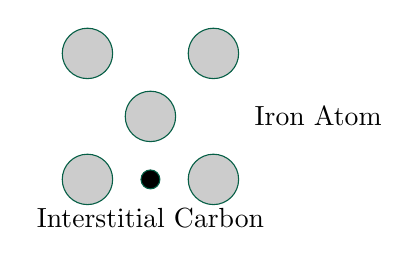
\begin{tikzpicture}[scale=0.8]
  % Draw a BCC lattice representation of iron
  \foreach \x in {0,2} {
    \foreach \y in {0,2} {
      \draw[fill=gray!40, draw=JourneyColor] (\x,\y) circle (0.4);
    }
  }
  \draw[fill=gray!40, draw=JourneyColor] (1,1) circle (0.4);
  \node[right] at (2.5, 1.0) {Iron Atom};
  
  % Draw a carbon atom in interstitial space
  \draw[fill=black, draw=JourneyColor] (1,0) circle (0.15);
  \node[below] at (1,-0.3) {Interstitial Carbon};
\end{tikzpicture}
\end{center}

\medskip
\textbf{Question 1.} Iron crystallizes in a body-centered cubic (BCC) or face-centered cubic (FCC) lattice. The carbon atoms are much smaller than iron atoms and occupy the small gaps between iron atoms (interstitial sites). Why does the presence of these tiny interstitial atoms make it harder for the planes of iron atoms to slide past one another?

\textbf{Question 2.} If we instead add nickel atoms, which are similar in size to iron, they substitute directly for iron atoms in the lattice. How does this substitutional doping modify the mechanical properties?

\textbf{Question 3.} Steel can be hardened by heating it to a high temperature and quenching it rapidly in water. What is happening to the atomic configuration during this rapid cooling?
\end{puzzlebox}

\newpage

% ─── Section: Exploration ────────────────────────────────────────────────────
\section{Part 2 --- Exploration}

\subsection{Step 1: Dislocations and Slip Systems}

\begin{problembox}
Theoretical calculations show that to slide one plane of atoms over another in a perfect crystal requires a shear stress $\tau_{\text{theo}} \approx G / 2\pi$, where $G$ is the shear modulus of the metal. For copper, $G \approx \SI{48}{GPa}$, which predicts a strength of $\sim \SI{7.6}{GPa}$. However, real copper crystals yield at a shear stress of less than \SI{1}{MPa}.
The explanation is that crystals deform not by sliding entire planes at once, but by propagating a line defect called a \newterm{dislocation}.

\begin{enumerate}[label=(\alph*)]
  \item An \newterm{edge dislocation} can be visualized as an extra half-plane of atoms inserted into the crystal lattice. Explain why propagating an edge dislocation requires breaking only one row of atomic bonds at a time, rather than an entire plane of bonds. Use a simple analogy (e.g., moving a rug by pushing a wrinkle across it).
  \item Slip occurs on specific crystallographic planes and in specific directions. The combination of a slip plane and a slip direction is called a **slip system**. Slip systems typically occur on the most densely packed planes and in the most closely packed directions. Why does the lattice require less energy to deform along these dense planes?
  \item For FCC metals (like copper or aluminum), the slip plane is $\{111\}$ and the slip direction is $\langle 110\rangle$. Show that there are 4 distinct $\{111\}$ planes and 3 distinct $\langle 110\rangle$ directions in each plane, giving a total of 12 slip systems. Why does this high number of slip systems make FCC metals highly ductile?
\end{enumerate}
\end{problembox}

\subsection{Step 2: Resolving Shear Stress (Schmid's Law)}

\begin{problembox}
Dislocations move in response to shear stress. If we apply a tensile force $F$ along the axis of a single crystal specimen, the force is resolved onto the slip plane (area $A$) and in the slip direction.

Let $\phi$ be the angle between the tensile axis and the normal to the slip plane, and let $\lambda$ be the angle between the tensile axis and the slip direction.

\begin{enumerate}[label=(\alph*)]
  \item Show that the area of the slip plane is $A_s = A_0 / \cos\phi$, where $A_0$ is the cross-sectional area of the crystal.
  \item Show that the component of the tensile force resolved in the slip direction is $F_s = F \cos\lambda$.
  \item Combine these results to prove **Schmid's Law** for the resolved shear stress $\tau$:
        \[
          \tau \;=\; \sigma \cos\phi \cos\lambda,
        \]
        where $\sigma = F / A_0$ is the applied tensile stress.
  \item What combination of angles $\phi$ and $\lambda$ yields the maximum resolved shear stress for a given tensile load? What is this maximum stress?
\end{enumerate}
\end{problembox}

\newpage

% ─── Section: Discovery ──────────────────────────────────────────────────────
\section{Part 3 --- Discovery}

\begin{discoverybox}
\textbf{Hardening Mechanisms}

To make a metal stronger, we must obstruct the motion of dislocations. Material scientists employ four main chemical and physical strategies to achieve this:

\begin{enumerate}
  \item \important{Solid Solution Hardening:} Introducing impurity atoms (substitutional or interstitial) creates local lattice strain fields. These strain fields interact with and pin dislocations, requiring a higher stress to move them.
  \item \important{Work Hardening (Strain Hardening):} Plastic deformation increases the density of dislocations. As dislocations multiply, they intersect and entangle, creating "forests" of dislocations that block each other's movement.
  \item \important{Precipitation Hardening:} Secondary phase particles are precipitated within the grain matrix by heat treatment. These particles force dislocations to either cut through them or bow around them (Orowan looping), increasing the yield stress.
  \item \important{Grain Boundary Strengthening (Hall-Petch effect):} Grain boundaries act as barriers to dislocation motion because the slip planes change direction at the boundary. Smaller grains mean more boundaries per unit volume, which increases strength.
\end{enumerate}
\end{discoverybox}

\newpage

% ─── Section: What This Is Called ────────────────────────────────────────────
\section{Part 4 --- What This Is Called}

\begin{namedconcept}{Mechanical Metallurgy}
\begin{itemize}
  \item \important{Burgers Vector ($\mathbf{b}$):} The vector representing the magnitude and direction of the lattice distortion associated with a dislocation.
  \item \important{Yield Strength ($\sigma_y$):} The stress at which a material transitions from elastic (reversible) deformation to plastic (permanent) deformation.
  \item \important{Hall-Petch Equation:} The empirical relation expressing yield strength as a function of average grain diameter $d$:
        \[
          \sigma_y \;=\; \sigma_0 + k_y d^{-1/2}.
        \]
  \item \important{Hume-Rothery Rules:} A set of empirical rules outlining the conditions under which two metals can form a substitutional solid solution (similar atomic size, same crystal structure, similar electronegativity, and valence).
\end{itemize}
\end{namedconcept}

\newpage

% ─── Section: Solved Exercises ───────────────────────────────────────────────
\section{Part 5 --- Solved Exercises}

\begin{problembox}
\textbf{Exercise:} A single crystal of a metal has a slip plane normal at $\phi = \ang{60}$ to the tensile axis and a slip direction at $\lambda = \ang{35}$ to the tensile axis. The critical resolved shear stress (CRSS) required to move dislocations is $\tau_{\text{crss}} = \SI{4.0}{MPa}$.
\begin{enumerate}
  \item Calculate the tensile stress $\sigma$ required to initiate plastic deformation.
  \item If the slip plane normal were perpendicular to the tensile axis ($\phi = \ang{90}$), what tensile stress would be required to yield the crystal? Interpret this result.
\end{enumerate}

\textbf{Solution:}
\begin{enumerate}
  \item Using Schmid's Law:
        \[
          \tau_{\text{crss}} \;=\; \sigma \cos\phi \cos\lambda.
        \]
        Solve for $\sigma$:
        \[
          \sigma \;=\; \frac{\tau_{\text{crss}}}{\cos\phi \cos\lambda}.
        \]
        Substitute the given values ($\cos\ang{60} = 0.5$ and $\cos\ang{35} \approx 0.819$):
        \[
          \sigma \;=\; \frac{4.0}{0.5 \times 0.819} \;=\; \frac{4.0}{0.4095} \;\approx\; \SI{9.77}{MPa}.
        \]
  \item If $\phi = \ang{90}$, then $\cos\phi = 0$. Schmid's Law yields $\tau = 0$ for any finite tensile stress $\sigma$. Therefore:
        \[
          \sigma \;=\; \frac{\tau_{\text{crss}}}{0} \;\to\; \infty.
        \]
        This means that no amount of tensile stress along this orientation can resolve a shear force on the slip plane. The slip system is "inactive," and the crystal cannot yield along this system.
\end{enumerate}
\end{problembox}

\newpage

% ─── Section: Problems ───────────────────────────────────────────────────────
\section{Part 6 --- Problems}

\begin{problembox}
\begin{enumerate}[label=\textbf{P\arabic*.}]
  \item \textbf{The Hall-Petch Analysis.}
  
        An alloy has a yield strength of $\sigma_{y1} = \SI{120}{MPa}$ when the grain size is $d_1 = \SI{100}{\mu m}$, and a yield strength of $\sigma_{y2} = \SI{220}{MPa}$ when the grain size is $d_2 = \SI{10}{\mu m}$.
        \begin{enumerate}[label=(\alph*)]
          \item Determine the material constants $\sigma_0$ and $k_y$ in the Hall-Petch equation.
          \item Predict the yield strength of the alloy if the grain size is refined to $d_3 = \SI{1.0}{\mu m}$ by severe plastic deformation.
        \end{enumerate}

  \item \textbf{Interstitial Solute Sizing.}
  
        Carbon occupies the octahedral interstitial sites in iron. The octahedral site radius in BCC iron is $r_{\text{oct}} \approx \SI{19}{pm}$, while the atomic radius of carbon is $r_{\text{C}} \approx \SI{77}{pm}$.
        \begin{enumerate}[label=(\alph*)]
          \item Calculate the local lattice strain $\epsilon = (r_{\text{C}} - r_{\text{oct}})/r_{\text{oct}}$.
          \item Explain how this strain leads to the formation of Cottrell atmospheres (carbon clusters around dislocation cores) and why this results in a sharp, distinct yield point in the stress-strain curve of mild steel.
        \end{enumerate}
\end{enumerate}
\end{problembox}

\newpage

% ─── Section: Deep Problems ──────────────────────────────────────────────────
\section{Part 7 --- Deep Problems}

\begin{deepbox}
\begin{enumerate}[label=\textbf{D\arabic*.}]
  \item \textbf{Lattice Strain Energy of a Dislocation.}
  
        A dislocation distorts the surrounding crystal lattice, creating elastic strain. We model a screw dislocation as a cylinder of length $L$ and radius $R$ in an isotropic elastic medium. The shear strain $\gamma$ at a distance $r$ from the dislocation line is given by:
        \[
          \gamma(r) \;=\; \frac{b}{2\pi r},
        \]
        where $b$ is the magnitude of the Burgers vector.
        \begin{enumerate}[label=(\alph*)]
          \item The elastic strain energy density (energy per unit volume) is $u = \frac{1}{2} G \gamma^2$, where $G$ is the shear modulus. Write $u(r)$ in terms of $G, b,$ and $r$.
          \item Integrate this energy density over the volume of a cylinder from a core radius $r_0 \approx b$ to the outer boundary of the crystal $R$ to show that the energy per unit length $E/L$ of a screw dislocation is:
                \[
                  \frac{E}{L} \;=\; \frac{G b^2}{4\pi} \ln\left(\frac{R}{r_0}\right).
                \]
          \item Estimate this energy per unit length (in J/m) for copper ($G = \SI{48}{GPa}$, $b = \SI{0.25}{nm}$, $R = \SI{1}{mm}$).
          \item Explain why the dependence of dislocation energy on $b^2$ (Frank's rule) implies that dislocations with smaller Burgers vectors are thermodynamically favored, and why dislocations decompose if $b^2 > b_1^2 + b_2^2$.
        \end{enumerate}
\end{enumerate}
\end{deepbox}

\newpage

% ─── Section: Reflection ─────────────────────────────────────────────────────
\section{Part 8 --- Reflection}

\begin{reflectionbox}
\textbf{Conceptual Reflection}

\begin{enumerate}
  \item **Defects as the Source of Reality:** Pure, perfect metal crystals are mechanically useless because they yield instantly. All practical structural materials depend entirely on the presence of imperfections --- dislocations, impurities, and grain boundaries --- to maintain their integrity. Discuss how this principle applies broadly in science: why are "ideal" systems often less robust than imperfect, real-world ones?
  \item **The Entropy of Structure:** Creating grain boundaries and dislocations increases the free energy of a metal because of the strain energy involved. Yet, we can maintain these high-energy defects indefinitely at room temperature because of kinetic barriers. Explain why materials science is fundamentally a study of metastable states rather than global thermodynamic equilibrium.
\end{enumerate}
\end{reflectionbox}

\vspace{1.4cm}
\begin{center}
{\color{JourneyColor}\rule{0.5\linewidth}{0.8pt}}\\[6pt]
{\small\color{JourneyColor}\textit{End of Journey 8, Module 8.3 --- Metals, Alloys, and Mechanical Properties}}\\[4pt]
{\small\color{JourneyColor}Continue to: \textbf{Module 8.4 --- Ceramics, Glasses, and Nanomaterials}}\\[6pt]
{\color{JourneyColor}\rule{0.5\linewidth}{0.8pt}}
\end{center}

\end{document}
